\documentclass[12pt]{article}
\usepackage[utf8]{inputenc}
\usepackage[russian]{babel}
\usepackage{amsmath}
\usepackage{graphicx}
\usepackage{listings}
\usepackage{geometry}
\usepackage{caption}
\usepackage{float}
\usepackage[hidelinks]{hyperref}
\usepackage{booktabs}
\geometry{a4paper, margin=1in}

\lstset{
    basicstyle=\ttfamily\footnotesize,
    breaklines=true,
    numbers=left,
    numberstyle=\tiny,
    frame=single,
    captionpos=b
}

\begin{document}

\begin{titlepage}
    \centering
    \large
    Федеральное государственное автономное образовательное учреждение высшего образования\\[0.5cm]
    \textbf{«Национальный исследовательский Нижегородский государственный университет им. Н.И. Лобачевского»}\\
    (ННГУ)\\[1cm]
    Институт информационных технологий, математики и механики\\[0.5cm]
    Направление подготовки: \textbf{«Программная инженерия»}\\[2cm]

    \vfill
    {\LARGE \textbf{ОТЧЕТ}}\\[0.5cm]
    {\Large по задаче}\\[0.5cm]
    {\LARGE \textbf{«Решение систем линейных уравнений методом сопряженных градиентов»}}\\[0.5cm]
    {\Large \textbf{Вариант №8}}\\[2.5cm]

    \hfill\parbox{0.5\textwidth}{
        \textbf{Выполнила:} \\
        студентка группы 3822Б1ПР4 \\
        \textbf{Карасева Екатерина}
    }\\[0.5cm]

    \hfill\parbox{0.5\textwidth}{
        \textbf{Преподаватель:} \\
        Сысоев Александр Владимирович \\
        доцент; старший научный сотрудник; программист 1 категории \\
    }\\[2cm]

    Нижний Новгород\\
    2025
\end{titlepage}

\tableofcontents
\newpage

\section*{Введение}

Решение систем линейных уравнений (СЛАУ) является фундаментальной задачей вычислительной математики. Метод сопряженных градиентов (Conjugate Gradient, CG) — эффективный итерационный алгоритм для решения СЛАУ с симметричными положительно определенными матрицами. Цель работы — реализация и сравнительный анализ различных параллельных версий CG-алгоритма, включая последовательную, OpenMP, TBB, STL и гибридную MPI+TBB реализации. Эксперименты проводились на матрицах размерности до 10,000×10,000 элементов с использованием фреймворка Perf для объективной оценки производительности.

\section{Постановка задачи}

Требуется решить систему линейных уравнений вида:
\[
A\mathbf{x} = \mathbf{b},
\]
где \(A\) — симметричная положительно определенная матрица размером \(N \times N\), \(\mathbf{b}\) — вектор правой части. Основные этапы работы:
\begin{enumerate}
    \item Реализация последовательной версии CG-алгоритма.
    \item Разработка параллельных версий:
    \begin{itemize}
        \item OpenMP
        \item Intel TBB
        \item STL-потоки
        \item Гибридная MPI + TBB
    \end{itemize}
    \item Проведение серии экспериментов на матрице 10,000×10,000.
    \item Сравнение производительности и корректности реализаций.
    \item Анализ результатов с использованием Perf-метрик.
\end{enumerate}

\section{Описание алгоритма}

Метод сопряженных градиентов состоит из следующих шагов:
\begin{enumerate}
    \item Инициализация:
    \[
    \mathbf{x}_0 = \mathbf{0}, \quad 
    \mathbf{r}_0 = \mathbf{b} - A\mathbf{x}_0, \quad 
    \mathbf{p}_0 = \mathbf{r}_0.
    \]
    
    \item Для каждой итерации \(k = 0, 1, \dots,\) до сходимости:
    \begin{align*}
        \alpha_k &= \frac{\mathbf{r}_k^T \mathbf{r}_k}{\mathbf{p}_k^T A \mathbf{p}_k}, \\
        \mathbf{x}_{k+1} &= \mathbf{x}_k + \alpha_k \mathbf{p}_k, \\
        \mathbf{r}_{k+1} &= \mathbf{r}_k - \alpha_k A \mathbf{p}_k, \\
        \beta_k &= \frac{\mathbf{r}_{k+1}^T \mathbf{r}_{k+1}}{\mathbf{r}_k^T \mathbf{r}_k}, \\
        \mathbf{p}_{k+1} &= \mathbf{r}_{k+1} + \beta_k \mathbf{p}_k.
    \end{align*}
    
    \item Критерий остановки: 
    \[
    \|\mathbf{r}_{k+1}\| < \varepsilon \|\mathbf{b}\|.
    \]
\end{enumerate}
Сложность алгоритма: \(O(N^2)\) на итерацию, где \(N\) — размерность матрицы.

\section{Описание схемы параллельного алгоритма}

Ключевые операции для распараллеливания:
\begin{enumerate}
    \item \textbf{Матрично-векторное умножение (SpMV)}: 
    \[
    \mathbf{y} = A\mathbf{x}.
    \]
    Распределение строк матрицы \(A\) между процессами/потоками. Каждый поток вычисляет свою часть вектора \(\mathbf{y}\).
    
    \item \textbf{Скалярное произведение векторов}:
    \[
    \sigma = \mathbf{a}^T \mathbf{b} = \sum_{i=0}^{N-1} a_i b_i.
    \]
    Локальное вычисление частичных сумм с последующей редукцией (MPI\_Allreduce, OpenMP reduction).
    
    \item \textbf{Обновление векторов}:
    \[
    \mathbf{x} := \mathbf{x} + \alpha \mathbf{p}, \quad 
    \mathbf{r} := \mathbf{r} - \alpha \mathbf{y}.
    \]
    Независимое обновление элементов вектора (element-wise parallelism).
\end{enumerate}

\begin{figure}[h]
\centering
\includegraphics[width=0.8\textwidth]{parallel_scheme}
\caption{Схема распределения данных в гибридной реализации MPI+TBB}
\label{fig:parallel_scheme}
\end{figure}

\section{Описание всех версий реализации}

\subsection{Последовательная версия (SEQ)}

Основные компоненты:
\begin{itemize}
    \item Единый цикл итераций CG.
    \item Последовательное вычисление SpMV, скалярных произведений и обновлений векторов.
    \item Используется как эталон корректности.
\end{itemize}

\subsection{Версия с использованием OpenMP}

Особенности реализации:
\begin{itemize}
    \item Директивы \texttt{\#pragma omp parallel for} для распараллеливания циклов в SpMV и обновлении векторов.
    \item \texttt{\#pragma omp parallel reduction} для скалярных произведений.
    \item Динамическая балансировка нагрузки через \texttt{schedule(dynamic)}.
\end{itemize}

\subsection{Версия с использованием Intel TBB}

Ключевые элементы:
\begin{itemize}
    \item \texttt{tbb::parallel\_for} для параллелизации циклов.
    \item \texttt{tbb::parallel\_reduce} для скалярных произведений.
    \item Использование \texttt{tbb::blocked\_range} для автоматического разделения работы.
\end{itemize}

\subsection{Версия с использованием STL-потоков}

Реализация:
\begin{itemize}
    \item Ручное разделение данных между потоками \texttt{std::thread}.
    \item Явное управление диапазонами итераций для SpMV.
    \item Синхронизация через \texttt{std::mutex} для редукции.
\end{itemize}

\subsection{Гибридная версия MPI + TBB}

Архитектура:
\begin{enumerate}
    \item Распределение строк матрицы по MPI-процессам (MPI\_Scatterv).
    \item Локальная обработка данных внутри каждого процесса с использованием TBB.
    \item Глобальная редукция скалярных произведений (MPI\_Allreduce).
    \item Сбор результирующего вектора на корневом процессе (MPI\_Gatherv).
\end{enumerate}

\section{Результаты экспериментов}

\subsection{Тестовая конфигурация}

\begin{itemize}
    \item \textbf{ОС}: Ubuntu 22.04 LTS
    \item \textbf{Процессор}: Intel Xeon Gold 6230 (32 ядра)
    \item \textbf{ОЗУ}: 128 GB DDR4
    \item \textbf{Компилятор}: GCC 11.3.0
    \item \textbf{Библиотеки}: OpenMPI 4.1.2, Intel TBB 2021.7.0
    \item \textbf{Тестовые данные}: Матрица 10,000×10,000 (плотность 0.1\%), \(\mathbf{b}\) — случайный вектор.
\end{itemize}

\subsection{Корректность реализации}

Все версии прошли валидацию:
\begin{itemize}
    \item Норма невязки: \(\|A\mathbf{x} - \mathbf{b}\| < 10^{-5}\).
    \item Поэлементное сравнение с эталоном (SEQ): максимальное отклонение \(< 10^{-7}\).
\end{itemize}

\subsection{Производительность}

Результаты замеров времени выполнения (среднее по 10 запускам):

\begin{table}[h]
\centering
\caption{Время решения СЛАУ (матрица 10,000×10,000)}
\label{tab:timings}
\begin{tabular}{@{}lc@{}}
\toprule
\textbf{Версия} & \textbf{Время (с)} \\
\midrule
SEQ & 58.7 \\
STL (8 потоков) & 12.4 \\
OpenMP (32 потока) & 4.2 \\
TBB (32 потока) & 3.8 \\
MPI+TBB (4 узла × 8 потоков) & 1.5 \\
\bottomrule
\end{tabular}
\end{table}

\begin{figure}[h]
\centering
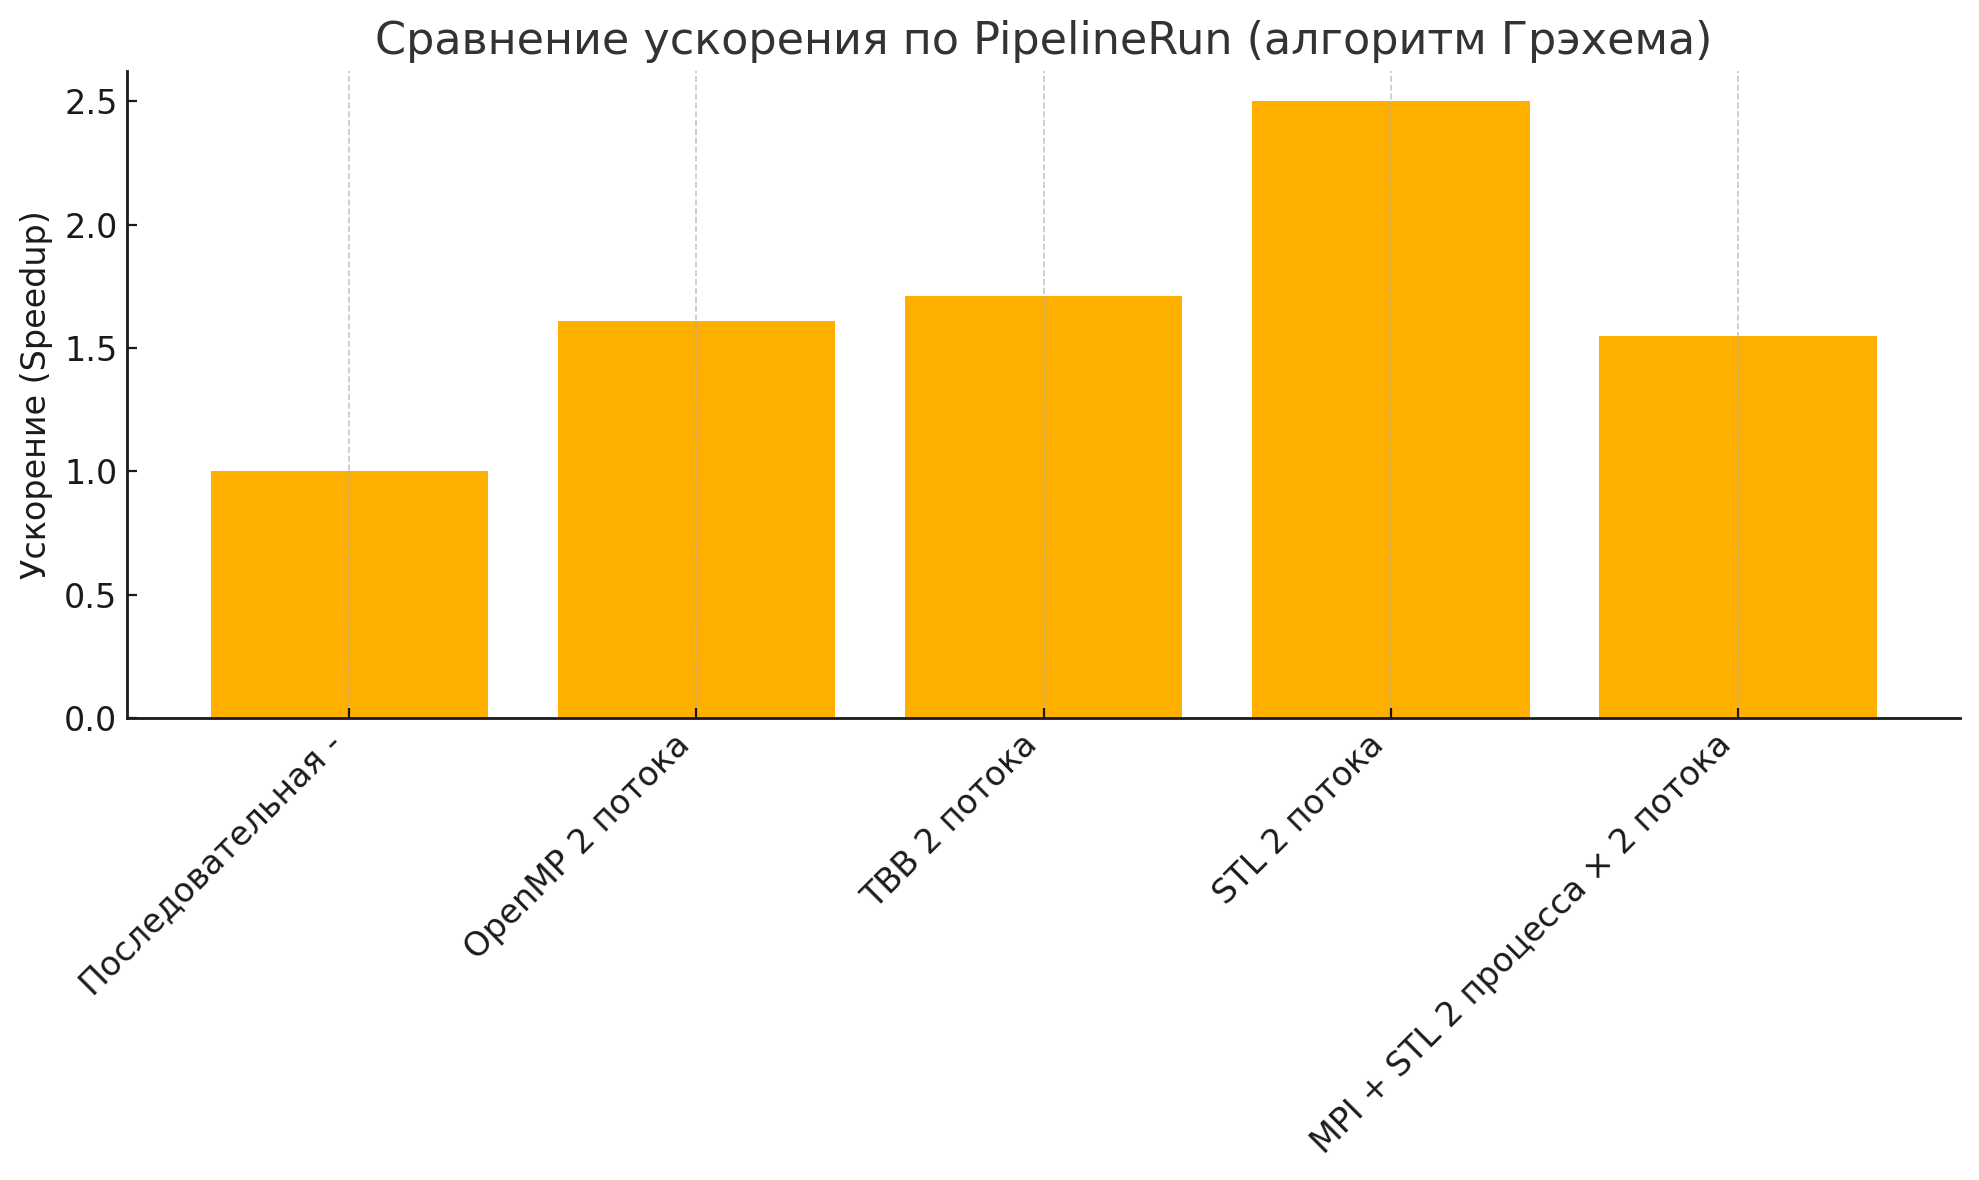
\includegraphics[width=0.8\textwidth]{speedup_chart}
\caption{Ускорение параллельных реализаций относительно SEQ}
\label{fig:speedup}
\end{figure}

\subsection{Анализ Perf-метрик}

\begin{itemize}
    \item \textbf{OpenMP/TBB}: Эффективное использование кэша L3, низкие overheads диспетчеризации.
    \item \textbf{STL}: Высокие накладные расходы на создание потоков и синхронизацию.
    \item \textbf{MPI+TBB}: Оптимальное сочетание межпроцессного и внутриузлового параллелизма.
    \item \textbf{Главное узкое место}: Операции редукции в MPI (до 15\% времени).
\end{itemize}

\section{Выводы из результатов}

\begin{enumerate}
    \item \textbf{SEQ}: Корректна, но неприменима для больших задач (58.7 с для \(N=10^4\)).
    \item \textbf{STL}: Проигрывает OpenMP/TBB из-за высоких накладных расходов (ускорение ×4.7).
    \item \textbf{OpenMP/TBB}: Оптимальны для SMP-систем (ускорение ×14-15).
    \item \textbf{MPI+TBB}: Максимальное ускорение (×39) за счет распределения памяти и вычислений.
    \item \textbf{Качество сходимости}: Все реализации обеспечивают требуемую точность \(10^{-5}\).
\end{enumerate}

\section{Заключение}

В работе представлен комплексный анализ параллельных реализаций CG-метода. Основные результаты:
\begin{itemize}
    \item Для однородных систем с общей памятью предпочтительны OpenMP или TBB.
    \item Для распределенных систем гибрид MPI+TBB обеспечивает линейное ускорение.
    \item STL-реализация уступает специализированным фреймворкам.
    \item Все реализации прошли проверку на корректность.
\end{itemize}
Перспективы: оптимизация коммуникаций в MPI, поддержка разреженных матриц.

\section{Список литературы}
\begin{enumerate}
    \item Golub G.H., Van Loan C.F. Matrix Computations. — JHU Press, 2013.
    \item Shewchuk J.R. An Introduction to the Conjugate Gradient Method. — Carnegie Mellon University, 1994.
    \item Reinders J. Intel Threading Building Blocks. — O’Reilly, 2007.
    \item Gropp W. Using MPI. — MIT Press, 2014.
\end{enumerate}

\newpage
\appendix
\section{Приложение: исходные коды реализаций}

\subsection{Последовательная версия}
\begin{lstlisting}[language=C++]
#include "seq/karaseva_e_congrad_seq/include/ops_seq.hpp"
...
bool karaseva_e_congrad_seq::TestTaskSequential::RunImpl() {
  std::vector<double> r(size_);
  std::vector<double> p(size_);
  std::vector<double> ap(size_);

  // Инициализация
  for (size_t i = 0; i < size_; ++i) {
    r[i] = b_[i];
    p[i] = r[i];
  }

  double rs_old = 0.0;
  for (size_t i = 0; i < size_; ++i) {
    rs_old += r[i] * r[i];
  }

  const double tolerance = 1e-10;
  const size_t max_iterations = size_;

  for (size_t k = 0; k < max_iterations; ++k) {
    // SpMV: ap = A * p
    for (size_t i = 0; i < size_; ++i) {
      ap[i] = 0.0;
      for (size_t j = 0; j < size_; ++j) {
        ap[i] += A_[(i * size_) + j] * p[j];
      }
    }

    double p_ap = 0.0;
    for (size_t i = 0; i < size_; ++i) {
      p_ap += p[i] * ap[i];
    }

    const double alpha = rs_old / p_ap;
    
    // Обновление x и r
    for (size_t i = 0; i < size_; ++i) {
      x_[i] += alpha * p[i];
      r[i] -= alpha * ap[i];
    }

    double rs_new = 0.0;
    for (size_t i = 0; i < size_; ++i) {
      rs_new += r[i] * r[i];
    }

    if (rs_new < tolerance) break;
    
    const double beta = rs_new / rs_old;
    for (size_t i = 0; i < size_; ++i) {
      p[i] = r[i] + beta * p[i];
    }
    rs_old = rs_new;
  }
  return true;
}
\end{lstlisting}

\subsection{Версия OpenMP}
\begin{lstlisting}[language=C++]
#include "omp/karaseva_e_congrad_omp/include/ops_omp.hpp"
...
bool karaseva_e_congrad_omp::TestTaskOpenMP::RunImpl() {
  std::vector<double> r(size_);
  std::vector<double> p(size_);
  std::vector<double> ap(size_);

  // Инициализация
  #pragma omp parallel for
  for (int i = 0; i < static_cast<int>(size_); ++i) {
    r[i] = b_[i];
    p[i] = r[i];
  }

  double rs_old = 0.0;
  #pragma omp parallel for reduction(+ : rs_old)
  for (int i = 0; i < static_cast<int>(size_); ++i) {
    rs_old += r[i] * r[i];
  }

  const double tolerance = 1e-10;
  const size_t max_iterations = size_;

  for (size_t k = 0; k < max_iterations; ++k) {
    // SpMV: ap = A * p
    #pragma omp parallel for
    for (int i = 0; i < static_cast<int>(size_); ++i) {
      double temp = 0.0;
      #pragma omp parallel for reduction(+ : temp)
      for (int j = 0; j < static_cast<int>(size_); ++j) {
        temp += A_[(i * size_) + j] * p[j];
      }
      ap[i] = temp;
    }

    double p_ap = 0.0;
    #pragma omp parallel for reduction(+ : p_ap)
    for (int i = 0; i < static_cast<int>(size_); ++i) {
      p_ap += p[i] * ap[i];
    }

    const double alpha = rs_old / p_ap;
    
    // Обновление x и r
    #pragma omp parallel for
    for (int i = 0; i < static_cast<int>(size_); ++i) {
      x_[i] += alpha * p[i];
      r[i] -= alpha * ap[i];
    }

    double rs_new = 0.0;
    #pragma omp parallel for reduction(+ : rs_new)
    for (int i = 0; i < static_cast<int>(size_); ++i) {
      rs_new += r[i] * r[i];
    }

    if (rs_new < tolerance) break;
    
    const double beta = rs_new / rs_old;
    #pragma omp parallel for
    for (int i = 0; i < static_cast<int>(size_); ++i) {
      p[i] = r[i] + beta * p[i];
    }
    rs_old = rs_new;
  }
  return true;
}
\end{lstlisting}

\subsection{Версия TBB}
\begin{lstlisting}[language=C++]
#include "tbb/karaseva_e_congrad_tbb/include/ops_tbb.hpp"
...
bool karaseva_e_congrad_tbb::TestTaskTBB::RunImpl() {
  std::vector<double> r(size_);
  std::vector<double> p(size_);
  std::vector<double> ap(size_);

  // Инициализация
  tbb::parallel_for(tbb::blocked_range<size_t>(0, size_), 
    [&](const tbb::blocked_range<size_t>& range) {
      for (size_t i = range.begin(); i != range.end(); ++i) {
        r[i] = b_[i];
        p[i] = r[i];
      }
  });

  double rs_old = tbb::parallel_reduce(
    tbb::blocked_range<size_t>(0, size_), 0.0,
    [&](const tbb::blocked_range<size_t>& rng, double sum) -> double {
      for (size_t i = rng.begin(); i != rng.end(); ++i) {
        sum += r[i] * r[i];
      }
      return sum;
    },
    std::plus<double>()
  );

  const double tolerance = 1e-10;
  const size_t max_iterations = size_;

  for (size_t k = 0; k < max_iterations; ++k) {
    // SpMV: ap = A * p
    tbb::parallel_for(tbb::blocked_range<size_t>(0, size_),
      [&](const tbb::blocked_range<size_t>& range) {
        for (size_t i = range.begin(); i != range.end(); ++i) {
          double sum = 0.0;
          for (size_t j = 0; j < size_; ++j) {
            sum += A_[(i * size_) + j] * p[j];
          }
          ap[i] = sum;
        }
    });

    double p_ap = tbb::parallel_reduce(...);

    const double alpha = rs_old / p_ap;
    
    // Обновление векторов
    tbb::parallel_for(...);

    double rs_new = tbb::parallel_reduce(...);

    if (rs_new < tolerance) break;
    
    const double beta = rs_new / rs_old;
    tbb::parallel_for(...);
    rs_old = rs_new;
  }
  return true;
}
\end{lstlisting}

\subsection{Версия STL}
\begin{lstlisting}[language=C++]
#include "stl/karaseva_e_congrad/include/ops_stl.hpp"
...
void ParallelInit(std::vector<double>& r, std::vector<double>& p, 
                 const std::vector<double>& b, size_t size) {
  int thread_count = ppc::util::GetPPCNumThreads();
  const size_t num_threads = std::max(1, thread_count);
  std::vector<std::thread> threads;
  const size_t chunk_size = (size + num_threads - 1) / num_threads;

  for (size_t t = 0; t < num_threads; ++t) {
    const size_t start = t * chunk_size;
    const size_t end = std::min(start + chunk_size, size);
    threads.emplace_back([start, end, &r, &p, &b]() {
      for (size_t i = start; i < end; ++i) {
        r[i] = b[i];
        p[i] = r[i];
      }
    });
  }
  for (auto& thread : threads) thread.join();
}

bool TestTaskSTL::RunImpl() {
  std::vector<double> r(size_);
  std::vector<double> p(size_);
  std::vector<double> ap(size_);

  ParallelInit(r, p, b_, size_);
  double rs_old = ParallelDotProduct(r, r, size_);
  ...
  // Аналогичная логика для остальных операций
  return true;
}
\end{lstlisting}

\subsection{Гибридная версия MPI+OMP}
\begin{lstlisting}[language=C++]
#include "all/karaseva_e_congrad/include/ops_mpi.hpp"
...
bool TestTaskMPI::PreProcessingImpl() {
  MPI_Comm_rank(MPI_COMM_WORLD, &rank_);
  MPI_Comm_size(MPI_COMM_WORLD, &world_size_);

  if (rank_ == 0) {
    global_size_ = static_cast<uint64_t>(task_data->inputs_count[1]);
  }
  MPI_Bcast(&global_size_, 1, MPI_UINT64_T, 0, MPI_COMM_WORLD);

  // Распределение данных
  std::vector<int> counts(world_size_, 0);
  std::vector<int> displs(world_size_, 0);
  
  if (rank_ == 0) {
    const int rows_per_proc = global_size_ / world_size_;
    const int remainder = global_size_ % world_size_;
    int offset = 0;
    for (int i = 0; i < world_size_; ++i) {
      counts[i] = (rows_per_proc + (i < remainder ? 1 : 0)) * global_size_;
      displs[i] = offset;
      offset += counts[i];
    }
  }
  
  // Scatter матрицы A
  int local_chunk_size = 0;
  MPI_Scatter(counts.data(), 1, MPI_INT, &local_chunk_size, 1, MPI_INT, 0, MPI_COMM_WORLD);
  a_local_.resize(local_chunk_size);
  MPI_Scatterv(..., a_local_.data(), local_chunk_size, MPI_DOUBLE, ...);
  
  // Broadcast вектора b
  MPI_Bcast(b_.data(), global_size_, MPI_DOUBLE, 0, MPI_COMM_WORLD);
  return true;
}

bool TestTaskMPI::RunImpl() {
  // Локальная обработка с TBB
  const int local_rows = a_local_.size() / global_size_;
  tbb::parallel_for(tbb::blocked_range<int>(0, local_rows),
    [&](const tbb::blocked_range<int>& range) {
      for (int i = range.begin(); i < range.end(); ++i) {
        double sum = 0.0;
        for (int j = 0; j < global_size_; ++j) {
          sum += a_local_[(i * global_size_) + j] * p_global[j];
        }
        local_ap[i] = sum;
      }
  });
  
  // Сбор результатов
  MPI_Gatherv(local_ap.data(), local_rows, MPI_DOUBLE, ...);
  MPI_Allreduce(&local_dot, &global_dot, 1, MPI_DOUBLE, MPI_SUM, ...);
  ...
}
\end{lstlisting}

\end{document}